\subsubsection{DSP Algorithms}

DSP algorithms allow for the mitigation or compensation of several
``impairments'' associated with coherent optical communication transmissions.
These include chromatic dispersion and polarization mode dispersion. By reducing
complexity in these systems, higher data rates can be
achieved\cite{dspcoherent}.

\par The receiver system described in Figure \ref{fig:dspcoherent} shows two fixed
equalizers, four ``butterfly-configured'' adaptive equalizers, and two phase
recovery units.

\begin{figure}[H]
	\centering
	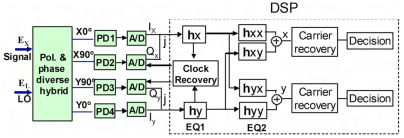
\includegraphics[width=0.8\textwidth]{images/dspcoherent}
	\caption{Generalised Digital Coherent Receiver\cite{dspcoherent}}
	\label{fig:dspcoherent}
\end{figure}

\par In order to compensate for chromatic dispersion, Fast Fourier Transform based
frequency-domain equalization can be used. Using this technique, the symbol rate
increases on a log scale, allowing for much lower complexity when compared with
a standard time-domain or frequency domain FIR filter. As such, within this
study, FFT-FDE based fixed equalizers are utilised.

\par Polarization-mode dispersion compensation is achieved using the four
adaptive equalizers. For this purpose, a T/2 spaced time-domain FIR filter
filter is used. This offers the best possible performance, however, if
complexity is a concern, a viable alternative is to use a 2T/3 FIR filter.
Using a constant modulus algorithm (CMA), the filter coefficients can be
chosen\cite{dspcoherent}.

\par The Viterbi-Viterbi (or Mth-power) method is used for the phase recovery
units. The incoming signal is raised to the $M^{th}$ power in order to remove
data modulation, and to attain the frequency offset between the transmit signal
and the local oscillator. Removing the frequency offset gives the frequency
recovered signal, to which the process is repeated in order to estimate the
phase noise, given by taking an average over multiple adjacent
symbols\cite{dspcoherent}.

\par Similar experiments have shown that the digital filtering described in
\cite{dspcoherent}, utilised in a coherent detection receiver system can achieve
high data transmission rates\cite{Savory_08}.
